%! TEX root = 'main.tex'

%\section{Experiments}

\section{Implementation}
\label{sec:implementation}

This section provides the implementation details and discusses the issues that we encountered during the development.



\subsection{Page Faults}


Exception handling is the primary method of \name. We leverage \texttt{SMAP} exception to notify the kernel-to-userspace access and next use exception to solve the read and write conflicts. Those events are all categorized as page faults. A page fault is a type of exception raised by the CPU when accessing a virtual page. The page ``fault'' mostly is not an error. It is the CPU's mechanism to implement virtual memory. For example, a page absence page fault is recoverable once the system assigns the physical page back.

We need to handle page fault exceptions before the system does.
Because the page fault caused by \texttt{SMAP} is fatal. It is not recoverable by design. Additionally, the followed exceptions that are related to the protection should not handle by the system either. We must also be careful with the exception that should send to the system, such as page absence. Because if we accidentally process those, it may cause the system to malfunction. To identify the cause of a page fault is not easy.  When page fault happens, the CPU pushes a 32-bit error code into the kernel stack with the format shown in~\autoref{fig:pagefaulterrorcode}.  Unfortunately, there is no exact error code regarding \texttt{SMAP}.  Still we can decide from the values in the kernel stack such as \texttt{CS:EIP}, \texttt{SS:ESP}, \texttt{EFLAGS} and the value from \texttt{CR2} and \texttt{CR3}.

\begin{figure}[th]
  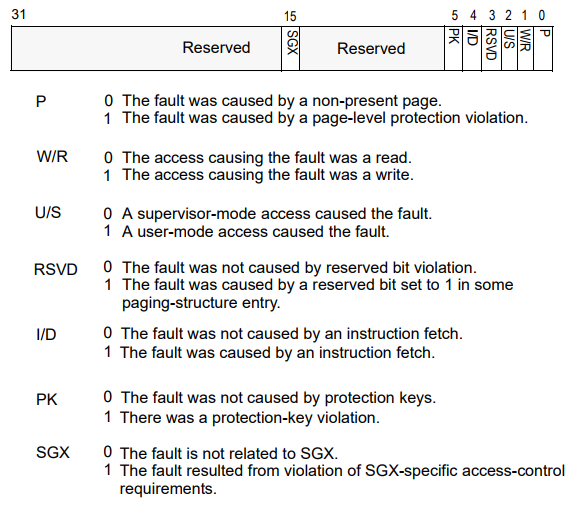
\includegraphics[width=0.47\textwidth]{figures/pagefaulterrorcode}
  \centering
  \caption{Page Fault Error Code.~\cite{intelinterrupt} Notice, there is no exact error code regarding \texttt{SMAP}. In the context of an \texttt{SMAP} exception, the \texttt{U/S} bit is zero, which indicates kernel-mode access. We still need to combine this information with the faulting address and \texttt{CS} segment register to confirm the cause.}
  \label{fig:pagefaulterrorcode}
\end{figure}



We need to filter out the irrelevant exceptions first. For example, \texttt{P:0} in the error code indicates the page absence, and we must pass it to the original page fault handler without any modification. We have not observed a \texttt{SMAP} exception on the invalid page, even though the error code may have combined bits. Other than that, \texttt{U/S:1} shows it is user-mode access, which will not cause \texttt{SMAP} exception.  The \texttt{Current Privilege Level (CPL)} in the \texttt{cs} segment register also reveals the context. Additionally, we keep track of the protected or relevant pages, which helps to identify the exceptions.



After filtering, ~\autoref{algo:pagefaulthandler} shows the basic algorithm to handle the \texttt{SMAP} and related exceptions.


\begin{algorithm}[ht]
\begin{algorithmic}[1]
\small
\Procedure{PageFaultHandler}{}

\State $address\gets cr2$ 
\State $pte\gets \Call{\textbf{GetPte}}{address}$
\State $teb\gets fs:0x18$

\If{SmapViolation}
	\State $pages[]\gets \Call{\textbf{AddPage}}{$address, pte, cr3, teb$}$
    	\State \Call{\textbf{SetPageKernel}}{pte}
    	\State \Call{\textbf{FlashTlb}}{address}
    	\State \Return{Re-execute}
\ElsIf{UserAccessProtectedPage}
	\If{error.WRITE}
    		\Repeat 
		\State \Call{\textbf{Sleep}}{}
        		\If{\Call{\textbf{CheckPtePermits}}{pte}}
        			\State \Return{Re-execute}
        		\EndIf
        	\Until{$count < 10$}
        	\State \Return{TerminateThread}
	\Else
    		\State \Call{\textbf{SetPgeUserReadonly}}{pte}
    		\State \Call{\textbf{FlashTlb}}{address}
        	\State \Return{Re-execute}
	\EndIf

%%\ElsIf{$user\_write\_readonlypage$}
%%	\If{\Call{HAS\_RECORD}{pte}}
%%    \EndIf

\EndIf
\State \Return{OriginalHandler}
   
\EndProcedure
\end{algorithmic}
\normalsize
\caption{Page Fault Handler}
\label{algo:pagefaulthandler}
\end{algorithm}



\textbf{\textit{Enable Interrut.}} The page fault exception is called through an \texttt{Interrupt Gate}~\cite{intelinterrupt}. Therefore, when entering the page fault handler, the CPU clears \texttt{EFLAGS:IF} automatically prevents subsequent interrupts from interfering with the handler's execution. Since we need to walk through the page table, it may access an invalid page, which triggers a nested page fault exception to bring the page back from disk. Therefore we need to set \texttt{EFLAGS:IF} before the page table walk.

\subsection{Hypervisor}


Intel \texttt{Virtual-Machine Extensions (VMX)} provides hardware-assistant virtualization, which adds 13 new instructions: \texttt{VMPTRLD}, \texttt{VMPTRST}, \texttt{VMCLEAR}, \texttt{VMREAD}, \texttt{VMWRITE}, \texttt{VMCALL}, \texttt{VMLAUNCH}, \texttt{VMRESUME}, \texttt{VMXOFF}, \texttt{VMXON}, \texttt{INVEPT}, \texttt{INVVPID}, and \texttt{VMFUNC}. \texttt{VMX} supports two modes, namely root and non-root mode, where in root mode runs the hypervisor, and virtual machines or called guest runs in non-root mode. On x86 architecture, the CPU has 4 protection rings, wherethe kernel runs at \texttt{ring 0}, the highest priority ring, and the user programs runs at \texttt{ring 3}, while the other two rings are not used. With VMX, the root model is often viewed as the \texttt{ring -1}. \texttt{VMXON}/\texttt{VMXOFF} enters/exits \texttt{VMX} mode. The \texttt{Virtual Machine Control Structure (VMCS)} is the most important data structure, which stores the data and state of one virtual CPU for one virtual machine. Each core in a physical CPU has a \texttt{VMCS} pointer. It points to the physical address of one \texttt{VMCS}. \texttt{VMPTRLD} loads the \texttt{VMCS} pointer from physical memory and makes it active and current. On contrary, \texttt{VMCLEAR} stores \texttt{VMCS} active states back to memory and makes it inactive. Although hypservisor fully aware the physical address of each \texttt{VMCS} but it can not modify them directly. All the operationgs on \texttt{VMCS} should go through instruction \texttt{VMREAD} and \texttt{VMWRITE}.



We do not use a bare-metal hypervisor because we create only one virtual machine, the current system, and do not need to emulate hardware. We use multiple \texttt{VMCS} that each represent one logical processor of the physical CPU and loads the logical processor's run-time state. Essentially, each processor exists in the system has its \texttt{VMCS}, hence no need to reload \texttt{VMCS} pointers.

The \texttt{VMCS} contains many data-fields that are related to aspects of a virtual machine. They are organized into six logical groups, namely, \texttt{Guest-state area}, \texttt{Host-state area}, \texttt{VM-execution control fields}, \texttt{VM-exit control fields}, \texttt{VM-entry control fields}, and \texttt{VM-exit information fields}. The last four groups compose \texttt{VMX controls}, which control the virtual machine's behavior such as when to exit to the hypervisor. In \texttt{VMX}'s term, \texttt{VM entry} is the transition into the \texttt{VMX} non-root operation while \texttt{VM exit} is the transition from the \texttt{VMX} non-root virtual machine to the VMX root  hypervisor. When VM exit, the processor stores its state into the \texttt{Guest-state area} and loads \texttt{Host-state area} into hardware. In contrast, it loads \texttt{Guest-state area} and stores \texttt{Host-state area} when entering the virtual machine. For our run-time load hypervisor, we set up those two areas mostly identical to the current CPU state but with different entry addresses, which, in root mode, serves the VM exit event handler's purpose. With that, we call \texttt{VMLAUNCH} respectively on each processor to enter the virtual machine. We control when the virtual machine exit through \texttt{VMX control} settings. To monitor the process context switch, we need the virtual machine exit on control register operations. In the event handler, the hypervisor can modify CPU state through \texttt{Guest-state area}, in this case, it is \texttt{CR4.SMAP}. After that, the hypervisor invokes \texttt{VMRESUME} to re-enter the virtual machine.

\subsection{Updating PTE}

We modify the bits in \texttt{PTE} to change a page's attribute. Updating system metadata such as the page table needs synchronization with other system components. Typically, the modifier should hold a global lock first. However, as a third-party kernel module, we do not have such information on Windows internal data.


%%\begin{lstlisting}[style=code, float]
%\begin{lstlisting}[style=code] 
%typedef struct _PTE_HARDWARE
%{
%	ULONG Valid : 1;
%	ULONG Write : 1;
%	ULONG Owner : 1;
%	ULONG WriteThrough : 1;
%	ULONG CacheDisable : 1;
%	ULONG Accessed : 1;
%	ULONG Dirty : 1;
%	ULONG Reserved : 1;
%	ULONG Global : 1;
%	ULONG Ignored: 3;
%	ULONG PageFrameNumber : 20;
%} PTE_HARDWARE, *PPTE_HARDWARE;
%
%typedef struct _PTE {
%	union {
%		ULONG Long;
%		PTE_HARDWARE Hard;
%	} u;
%} PTE, *PPTE;
%\end{lstlisting}

\begin{figure}[th]
  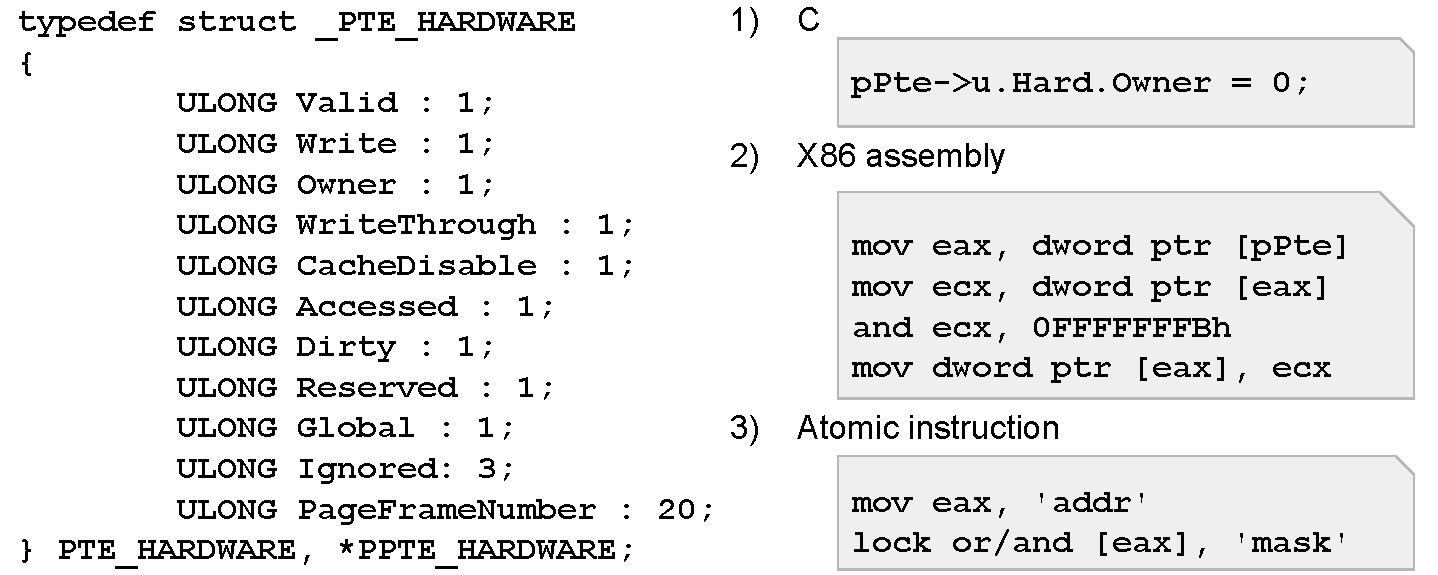
\includegraphics[width=0.47\textwidth]{figures/ptestructcode}
  \centering
  \caption{Left: PTE structure defined in C. Right: C code for changing one bit in the PTE structure, the corresponding assembly code generated by Microsoft C/C++ compiler, and the atomic instructions that serve the same purpose.}
  \label{fig:ptestruct}
\end{figure}


In a typical kernel-level TOCTOU attacking scenario, the attacker races with the kernel at full speed, so will our mitigation triggered. We modify the page table rapidly. Hence we need to make our operation as atomic as possible. ~\autoref{fig:ptestruct} shows the \texttt{PTE} data structure defined in C on a 32-bit system. The C code at \texttt{\textcircled{1}} changes the \texttt{Owner} a.k.a \texttt{U/S} bit to zero, which makes it a kernel-mode page. \texttt{\textcircled{2}} is the assembly code generated by a compiler, where once C statement needs three assembly instructions. However, during the three instructions, the current thread may be interrupted, or other threads may also update the same \texttt{PTE} due to the race condition, which occurs multiple times when we test the exploit agast \name. We use the locked atomic instruction~\cite{intelmanualchapter8} instead of the compiler-generated assembly code, as shown at \texttt{\textcircled{3}}. It guarantees that the update on one \texttt{PTE} is intact. 

In the future, if the operating system takes such mitigation into its source tree, it will solve such a synchronization issue entirely.

\subsection{TLB Flushing}
%A translation lookaside buffer(TLB), as mentioned earlier, is a memory cache that is used to store the mappings between virtual pages and physical pages. Different than data cache, TLB is not entirely transparent to the operating system. When operating system updates page tables, corresponding TLB entries need to be invalidated.
%
%Instruction "INVLPG" is used to invalidate a TLB entry. It has a source operand which is a virtual memory address. "INVLPG" only invalidate TLB entries on the current CPU, so on multiple processor system, we need to execute it on every processor that has the same TLB entry. To do do, we need to issue an inter-processor interruption(IPI) to inform all the CPU cores in the system.
%
%IPI allows a processor to send interrupt signals to other processors. It's different than normal "interrupt" which go through an IRQ line. IPI signal needs to be sent via the advanced programmable interrupt controller(APIC) bus which connects all the local APIC of every CPU core.
%
%In our implementation, we actually reuse some of the functionality from Windows operating system to issue the IPI for TLB flushing. Because Windows' MMU also need the same function to flush TLB, we found the address of the related internal functions at run-time, call it when we update a PTE. 
%



When we apply our mitigation on real hardware instead of a virtual machine, one crucial issue is the need to flush the TLB.  Translation Lookaside Buffer (TLB) is a memory cache used to reduce the time taken to access a virtual memory location. It stores the recent translations of virtual memory to physical memory. Different than data cache, TLB is not entirely transparent to the operating system. When the operating system updates a page table entry, the corresponding TLB entry needs to be invalidated.

Instruction INVLPG invalidates a TLB entry. It only has a source operand, which is a virtual memory address. INVLPG only affects the current CPU. However, on a multiple processor system, each processor core has its TLB. Therefore we need to do this on every core. For this purpose, we need to issue intel-processor interruption (IPI) to each core through APIC. Symmetric multiprocessing (SMP) system uses IPI messages to distribute interrupts among the processors in the system or execute system-wide functions such as booting up processors or distributing work among a group of processors. 

Intel's Advanced Programmable Interrupt Controller (APIC) is a family of interrupt controllers. It is more advanced than Intel's 8259 Programmable Interrupt Controller (PIC). Nowadays, SMP systems with multiple processors utilize APIC. The APIC is a split architecture design, with a local APIC usually integrated into the processor and an optional I/O APIC on a system bus. The local APIC performs two primary functions for the processor:
It receives interrupts from the processor's interrupt pins, internal sources, and an external I/O APIC. It sends these to the processor core for handling.
It sends and receives IPI messages to and from other logical processors on the system bus in multiple-processor systems.
The external I/O APIC is part of Intel's system chipset. It is responsible for receiving interrupts generated by system hardware and I/O devices and forwarding them to the local APIC as interrupt messages. A processor can generate IPIs by programming the interrupt command register (ICR) in its local APIC. Writing to the ICR generates an IPI message on the system bus or the APIC bus. When the target processor receives an IPI message, its local APIC handles the message automatically using information included in the message such as vector number and trigger mode. The IPI mechanism sends interrupts for a specific vector number, and special-purpose interrupts to processors on the system bus. Local APIC registers are memory-mapped to a 4-KByte region of the processor's physical address space with an initial starting address of EFF00000H. The software interacts with the local APIC by reading and writing its registers. It also can change the initial mapping to a different 4-KByte region for all the local APICs. The presence of a local APIC can be detected using the CPUID instruction. Execute CPUID with source operand of 1 in the EAX register, then bit 9 of returned feature flags in EDX register indicate a local APIC.


\begin{figure}[th]
  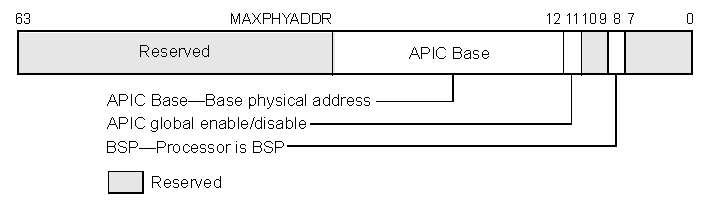
\includegraphics[width=0.40\textwidth]{figures/ia32apicbase}
  \centering
  \caption{\texttt{IA32\_APIC\_BASE} MSR}
  \label{fig:ia32apicbase}
\end{figure}

There is only one MSR associated with local APIC, \texttt{IA32\_APIC\_BASE}. As shown in~\autoref{fig:ia32apicbase}, the BSP flag indicates if the processor is the bootstrap processor (BSP); ``APIC global enable/disable'' enables/disables the APIC; APIC base specifies the base address of the APIC registers. This 24-bit value needs to be extended by 12 bits at the low end to form the base address. As formerly mentioned, this value by default is 0xFEE00000.

The primary local APIC facility for issuing IPIs is the interrupt command register (ICR), as shown in~\autoref{fig:icr}. It is a 64-bit local APIC register that allows the operating system to specify and send IPIs to processors in the system.


\begin{figure}[th]
  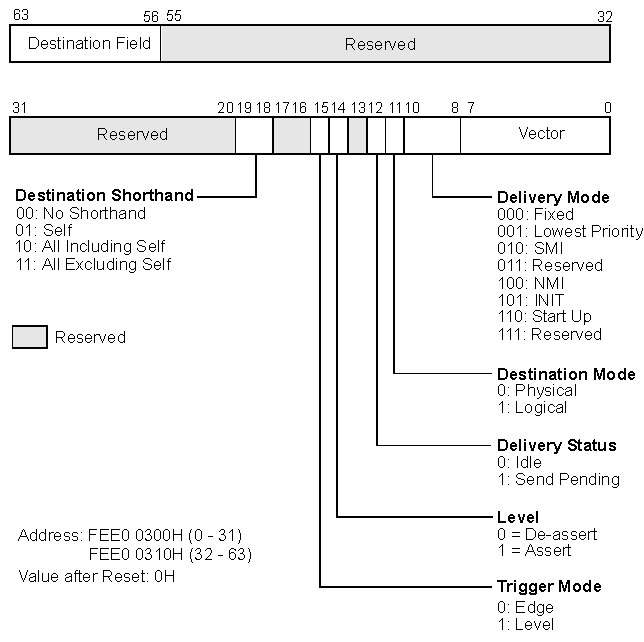
\includegraphics[width=0.40\textwidth]{figures/icr}
  \centering
  \caption{Interrupt Command Register (ICR)}
  \label{fig:icr}
\end{figure}

In this project, we find a Windows kernel internal function, KeFlushSingleTb(). It sends IPI to all processors to invalid a particular TLB entry, as mentioned above. The hardware abstraction layer (HAL) eventually sends the IPI, so the kernel does not need to mind the actual hardware differences.


\subsection{Crashing a Faulty Thread}

As mentioned earlier, to solve the problem that a user thread tries to write a protected page, instead of crashing the thread immediately, our approach is to hold the thread for some milliseconds, waiting for the function to end. To avoid any deadlock or blockage caused by a faulty program, we only allow for several retries. 

Since it is troublesome to call a series of undocumented functions to handle exceptions. We choose to let the operating system terminating it. We clears ``p'' bit of the corresponding PTE as well as changing the error code to a value that indicates ``accessing an invalid page'' instead of ``writing an read-only page''. Because we can't synchronize with MMU, when we passing the exception to the original page fault handler, the PTE's attributes could be changed within the short period of time due to another SMAP exception, this could happen especially in the attacking scenario. 

%global hook, it may use shared memory,  before put it here, probably should figure out how page permits works on shared page


\subsection{Special Cases}
We assume 32bit Windows operating system use the default 2G/2G user/kernel split where user space is below 0x7FFFFFFF. More precisely, a kernel variable MmUserProbeAddress contains the highest possible address for user data, which is set to 0x7FFF0000. And we learn that one page locates at 0x7FFE0000 is defined as \texttt{USER\_SHARED\_DATA}. It's a shared page between user mode and kernel mode, meaning the same physical page is mapped both at 0x7FFE0000 and 0xFFDF0000. It's a read-only page and contains a lot of process settings such as system time. Kernel needs to read this page a lot. We treat such page specially to improve performance. 


